\documentclass{article}

\usepackage{amsmath}
\usepackage{amssymb}
\usepackage{geometry}
\usepackage{fancyhdr}
\usepackage{graphicx}
\usepackage{array}
\usepackage{multirow}
\usepackage{tikz}
\usepackage{booktabs}
\usepackage{float}



% for custom subsection
\usepackage{titlesec}
% package for enumerate with letters
\usepackage{enumitem}

\titleformat{\subsection}
  {\normalfont\fontfamily{phv}\fontsize{14}{17}}{\thesubsection}{1em}{}

\geometry{margin=1in}
\pagestyle{fancy}
\fancyhf{}
\rhead{Kyle Wodehouse}
\lhead{MSEG201}
\chead{Homework 1}
\title{\bfseries Homework 1}
\author{Kyle Wodehouse}
\rfoot{\thepage}
% 1 -> 5 from least to most descriptive
\setcounter{tocdepth}{1}

\begin{document}
\maketitle

\section{Syllabus Review}

\begin{enumerate}[label=(\alph*)]
    \item 207 Dupont Hall 
    \item 6 homework assignments
    \item 17 at very least. 
    \item 'analyze and select an appropriate material for a given application' and 'select an approproate method to characterize the structure or properties of a material.'
\end{enumerate}

\section{Bonding Energy}

% import figure

\subsection*{a.}

\begin{figure}[h]
    \centering
    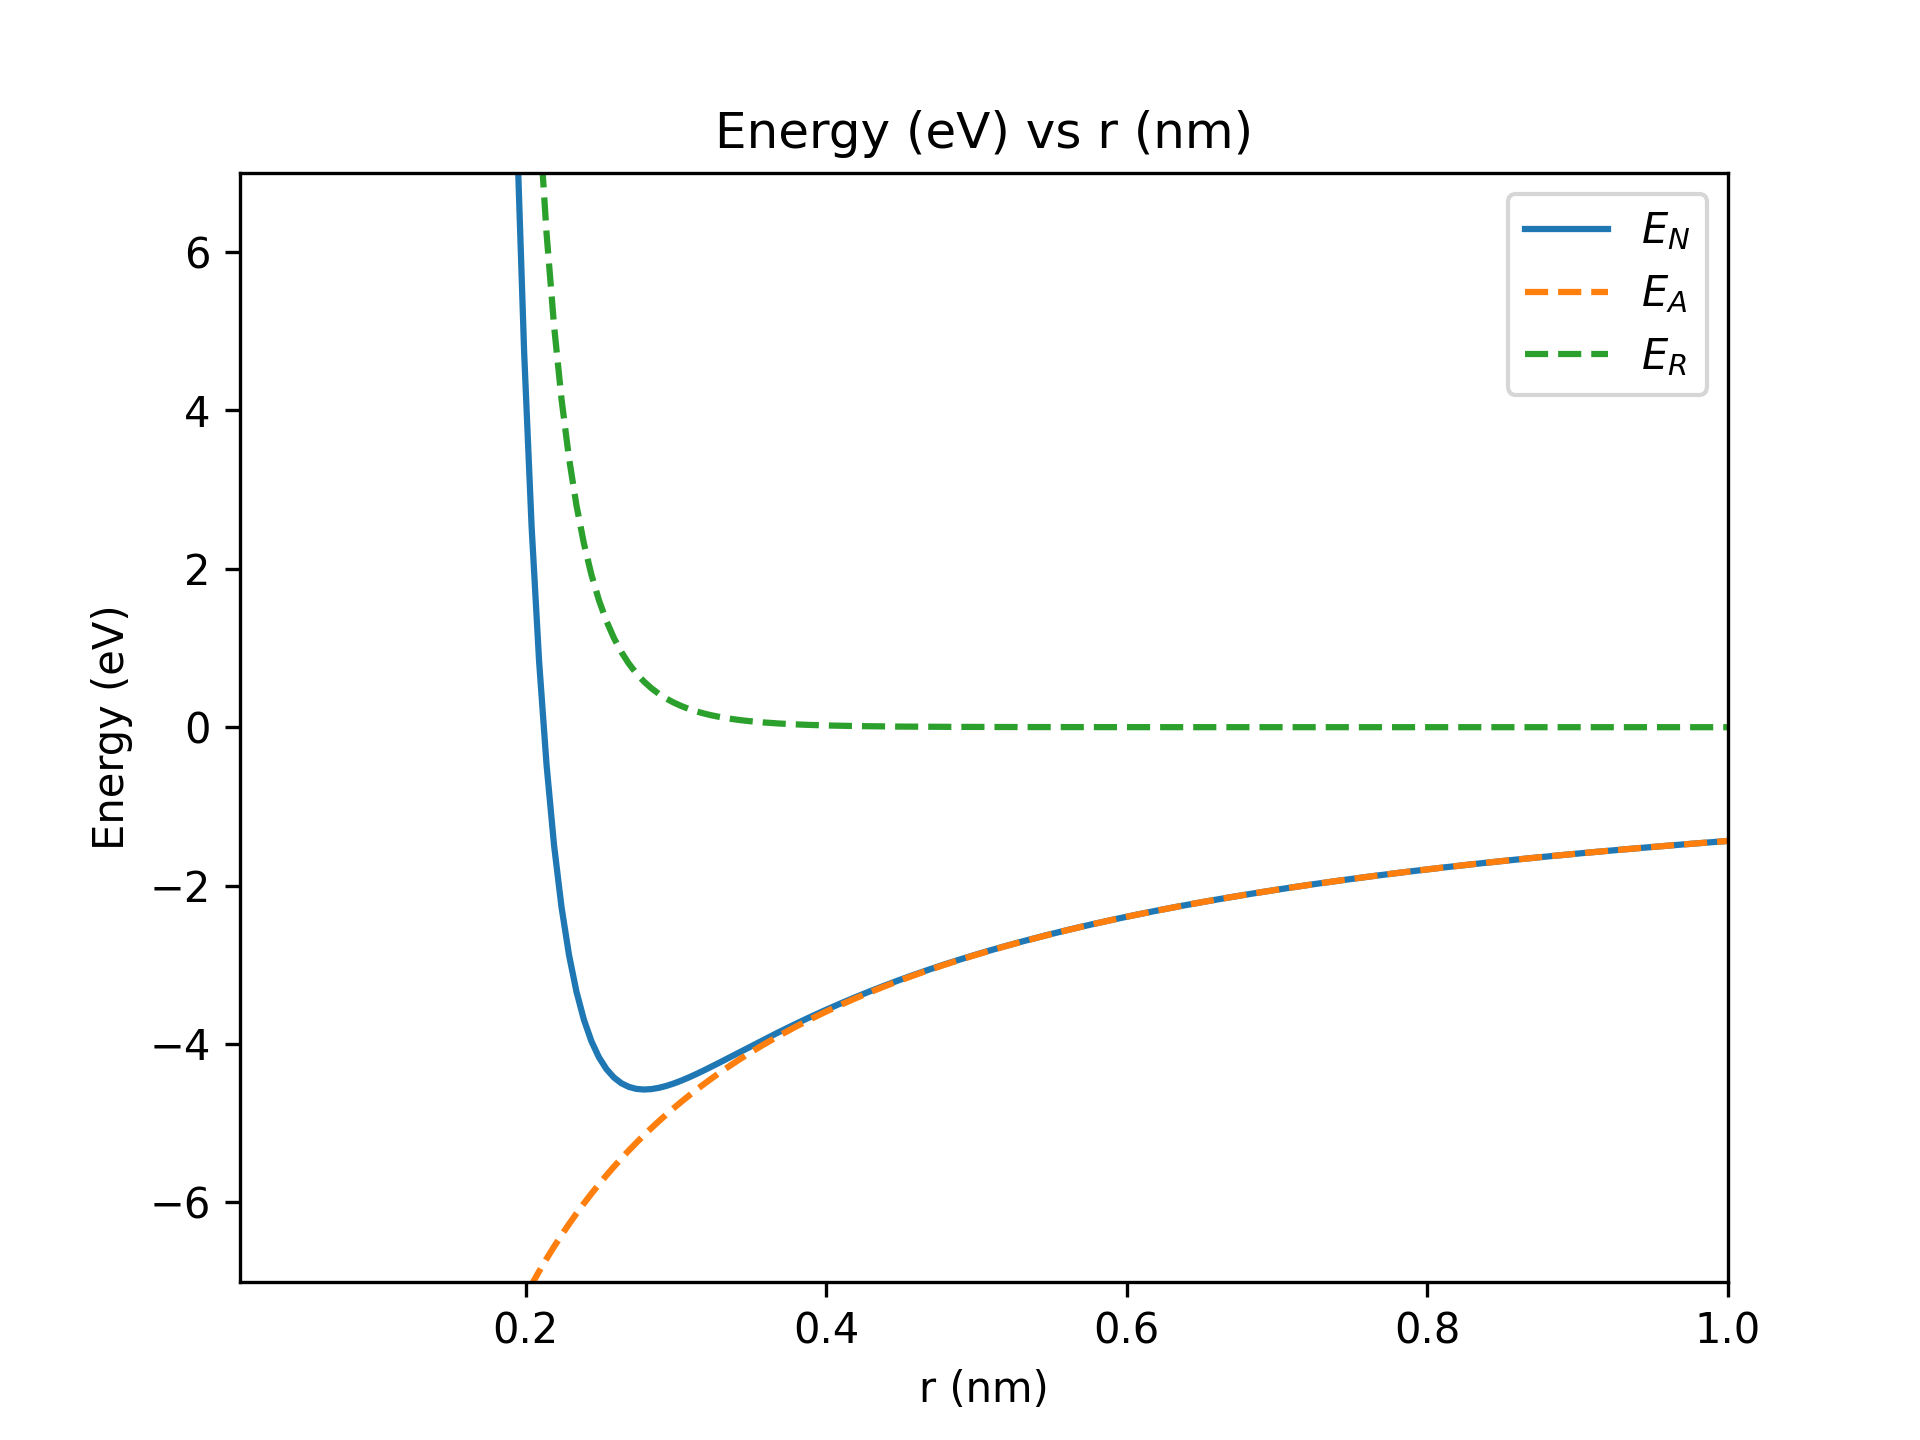
\includegraphics[width=0.6\textwidth]{2a.png}
    \caption{K$^+$ and Cl$^-$ energy profile}
\end{figure}

\subsection*{b.}

\begin{figure}[h]
    \centering
    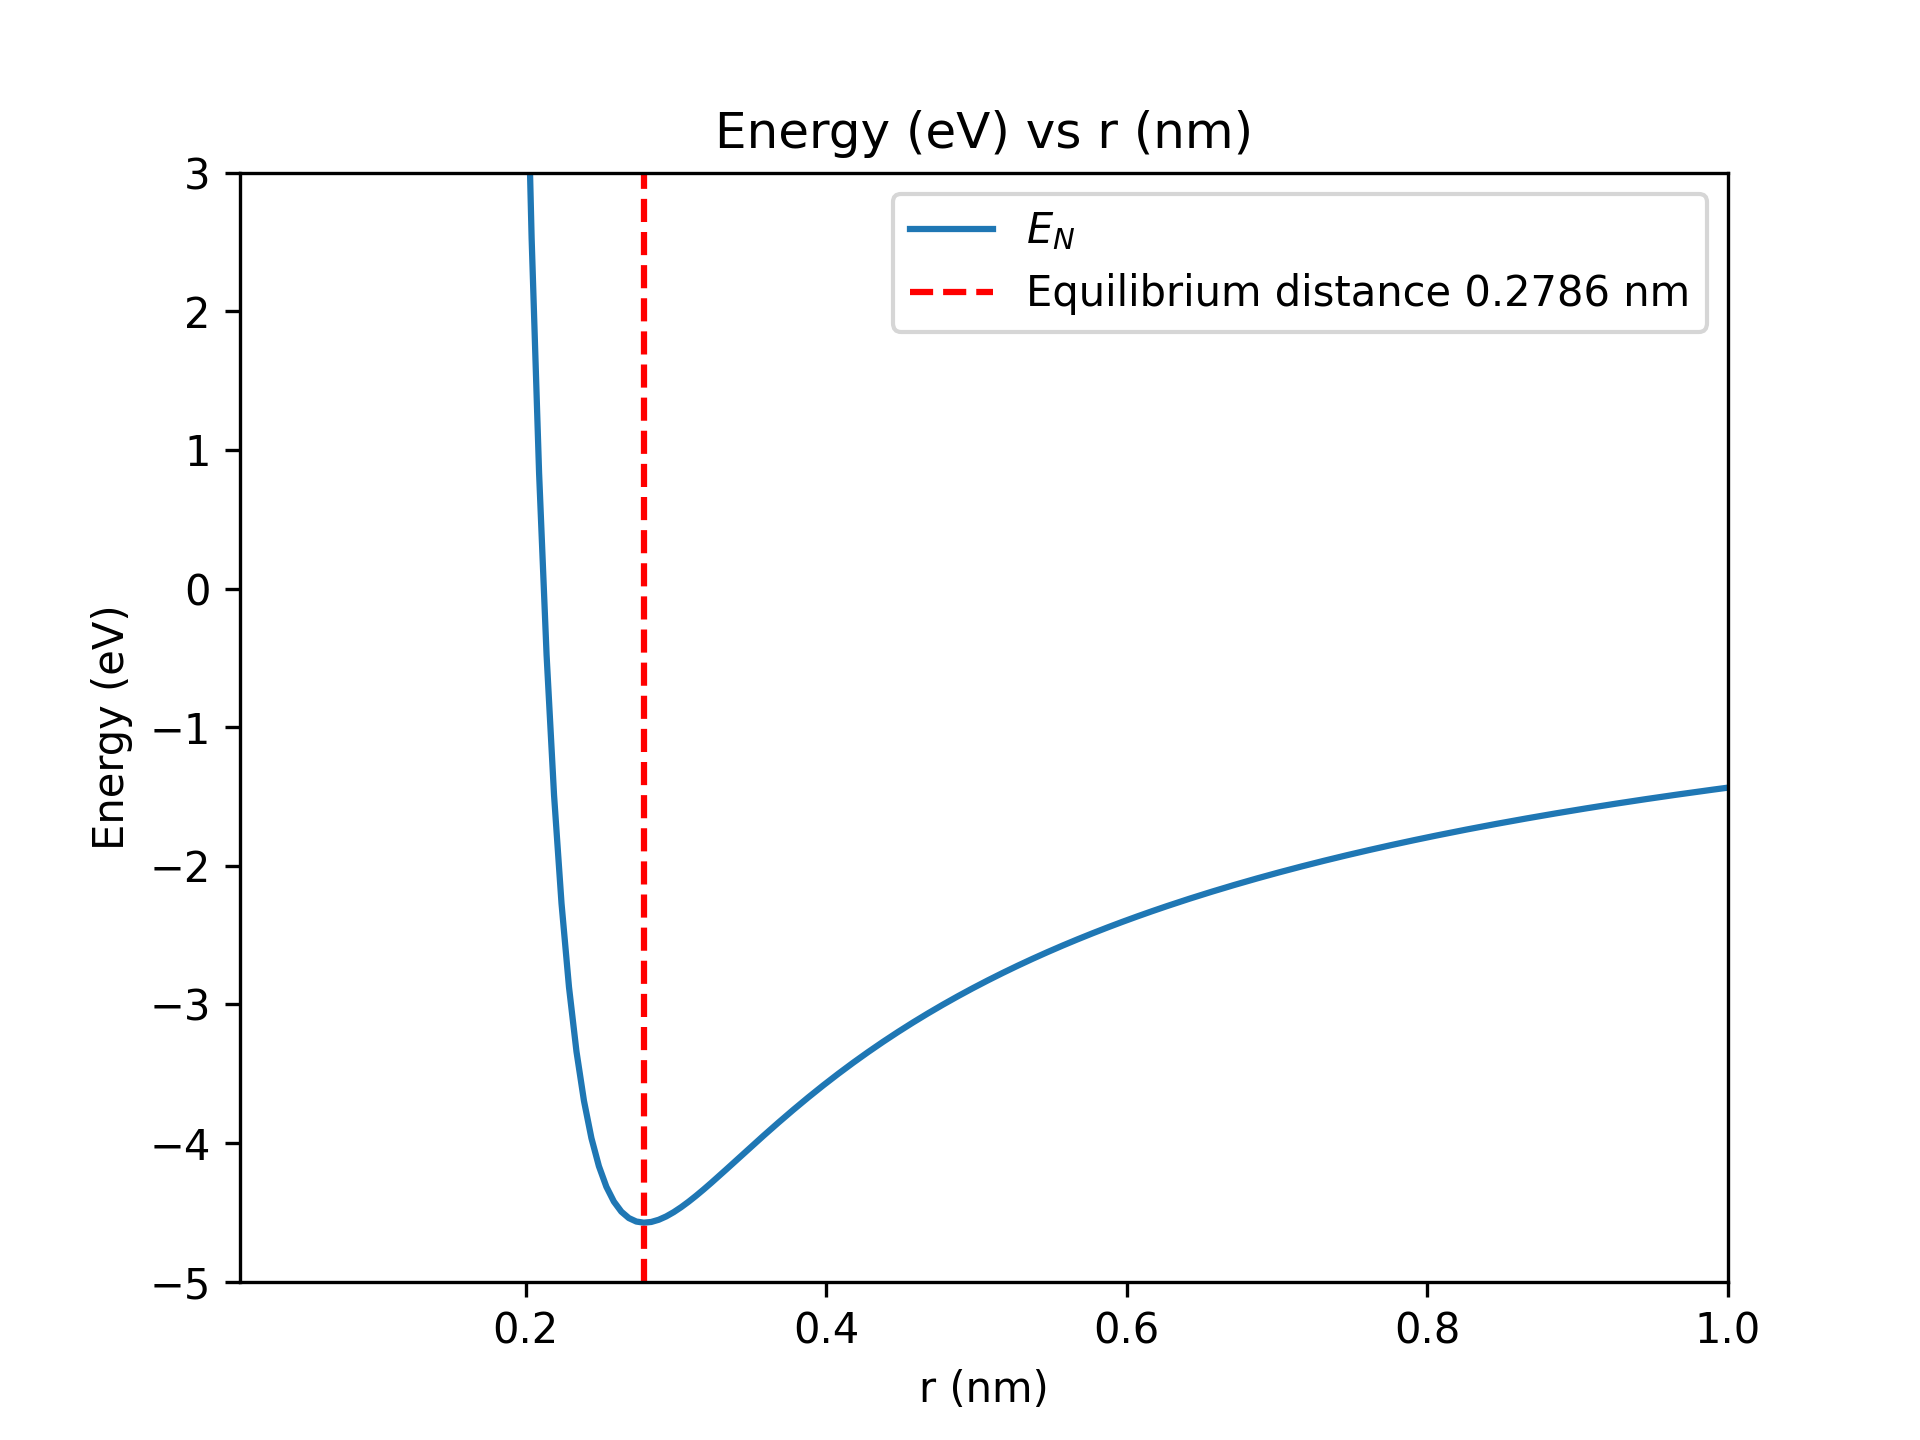
\includegraphics[trim=0cm 0cm 0cm 0cm, clip, width=0.75\textwidth]{2b.png}
    \caption{K$^+$ and Cl$^-$ energy profile with local minimum displayed}
\end{figure}

for this one I used some python code to put a vertical line at the distance where energy is minimized--\textit{the equlibrium bond length will be when the energy is at a local minimum}. To be a little more rigorous and get some more digits I also loaded up desmos and graphically found the minimum on there as well.

\begin{figure}[H]
    \centering
    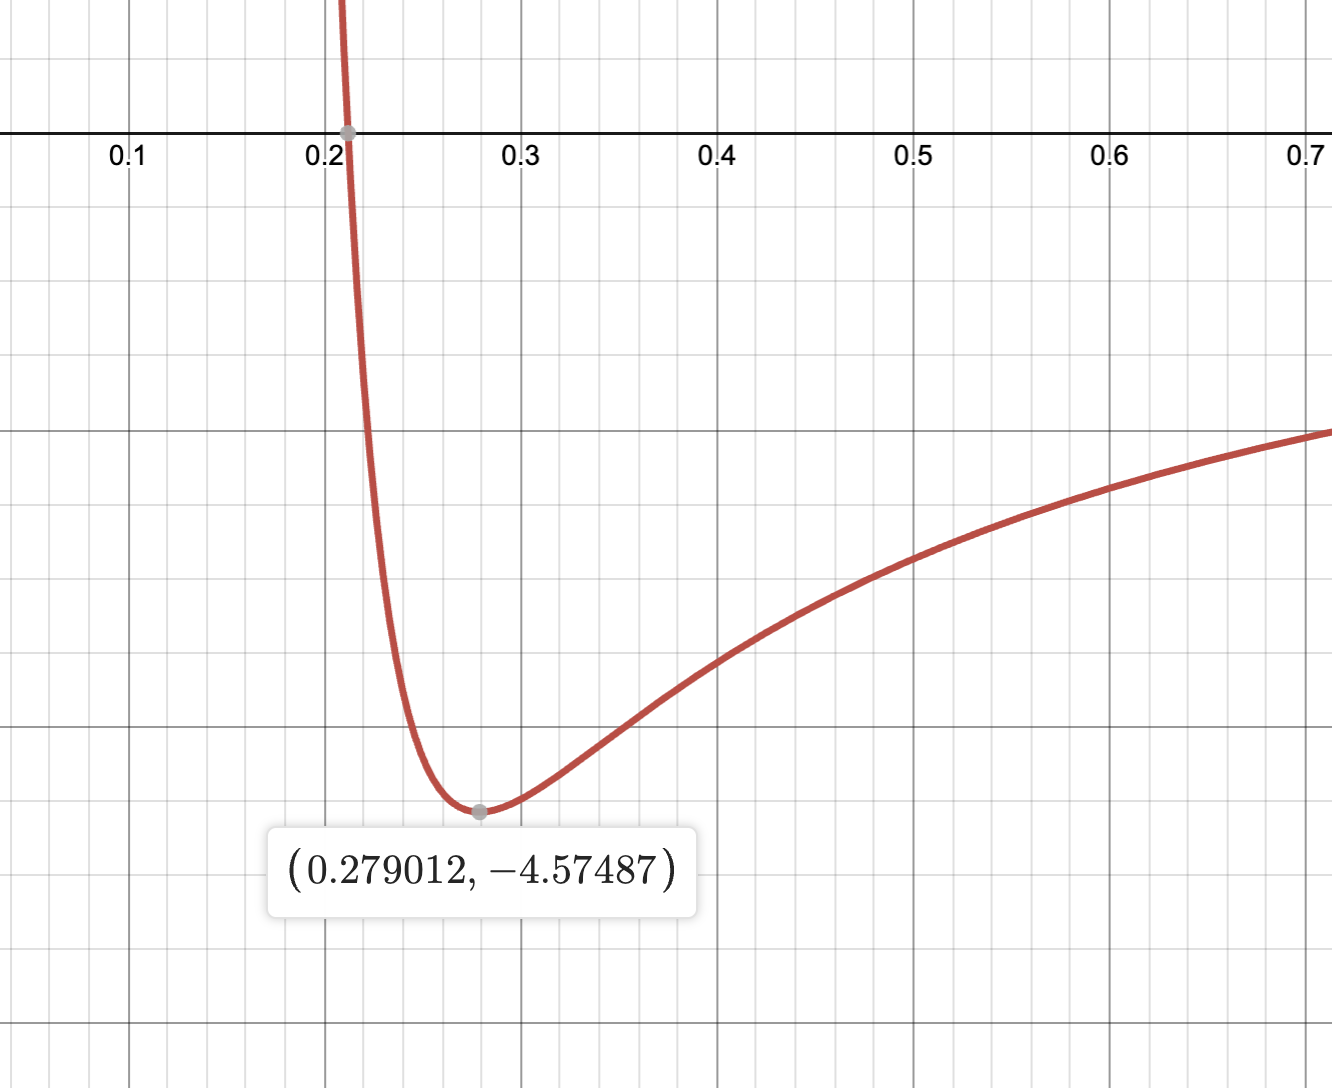
\includegraphics[trim=0cm 0cm 0cm 0cm, clip, width=0.75\textwidth]{2b_desmos.png}
    \caption{K$^+$ and Cl$^-$ energy profile on desmos with local minimum displayed}
\end{figure}


From the desmos graph, the equlibrium spacing and the magnitude of the bonding energy are 0.279 nm and -4.57 eV respectively.

\subsection*{c.}

To mathematically calculate it we can take the derivitive, set it equal to zero, and solve for $r$ and then plug that into the original equation to get the energy. 

At equlibrium spacing,
\begin{align*}
    \frac{dE}{dr} &= 0 \\
    \frac{d}{dr} \left( - 
    \frac{A}{r} + \frac{B}{r^9} \right) &= 0 \\
    \frac{A}{r^2} - \frac{9B}{r^{10}} &= 0 \\
    A = \frac{9B}{r^8} \\
    r^8 &= \frac{9B}{A} \\
    r &= \left( \frac{9B}{A} \right)^{1/8} \\
     &= \left( \frac{9 \times (5.86 \times 10^{-6})}{1.436} \right)^{1/8} \\
        &= 0.279 \text{ nm}
\end{align*}

Now we can plug this into the original equation to get the energy at the equlibrium spacing:

\begin{align*}
    E &= - \frac{1.436}{0.279} + \frac{5.86 \times 10^{-6}}{(0.279)^9} \\
    &= -4.57 \text{ eV}
\end{align*}

\section{Miller Indices: Directions}

\subsection*{a. [001]}

\begin{figure}[H]
    \centering
    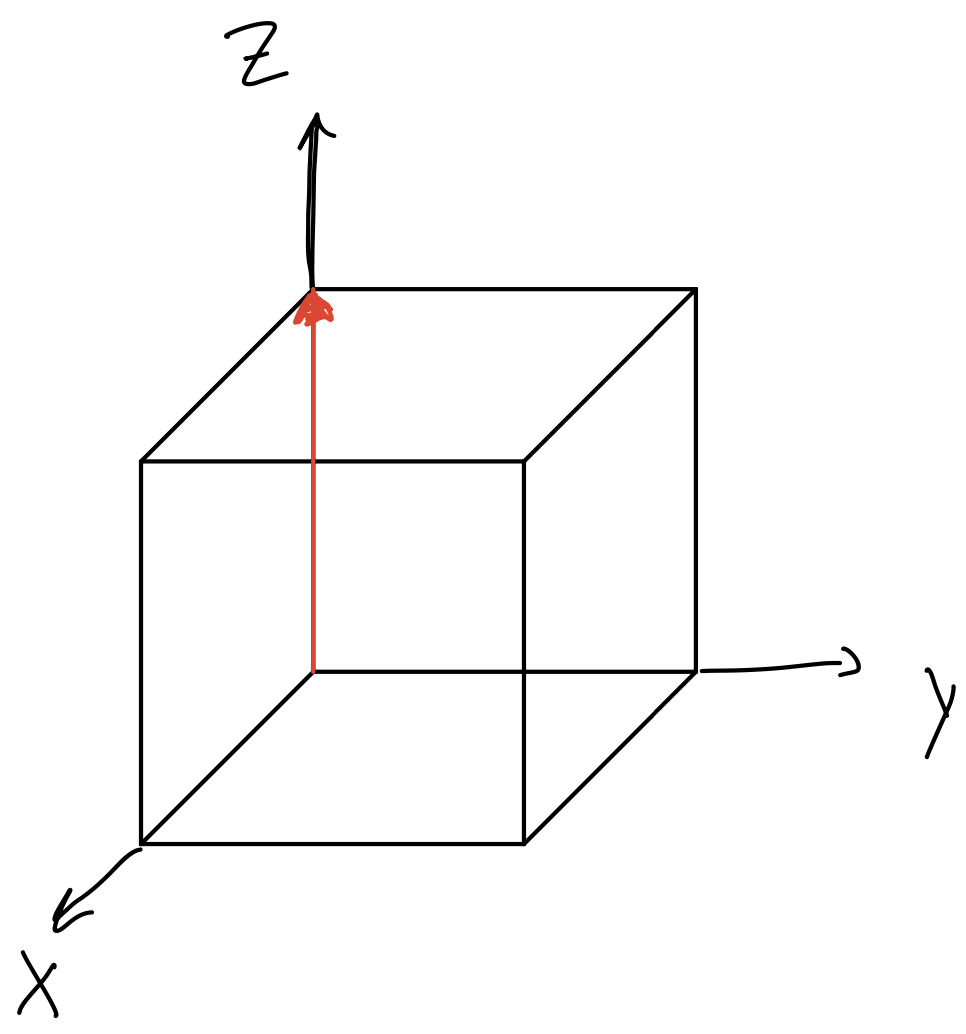
\includegraphics[width=0.5\textwidth]{3a.png}
\end{figure}

\subsection*{b. [102]}

\begin{figure}[H]
    \centering
    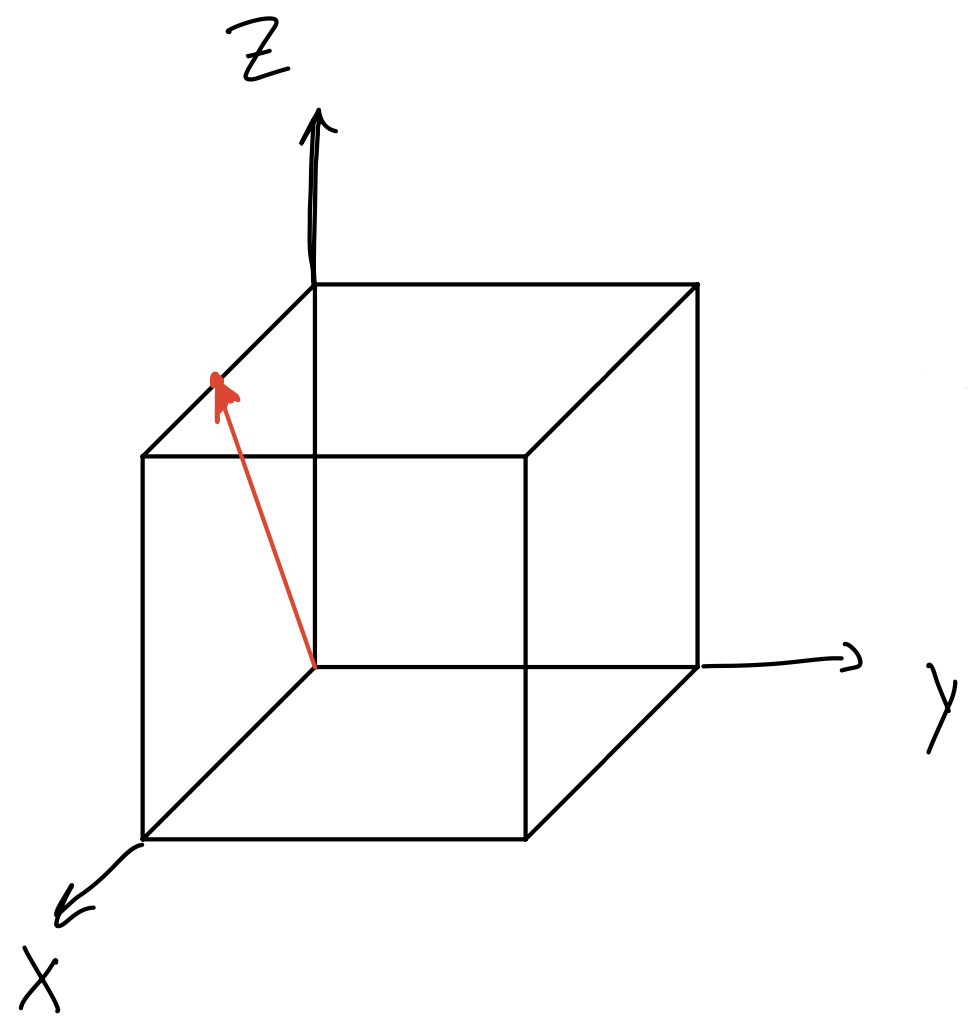
\includegraphics[width=0.5\textwidth]{3b.png}
\end{figure}


\subsection*{c. [012]}

\begin{figure}[H]
    \centering
    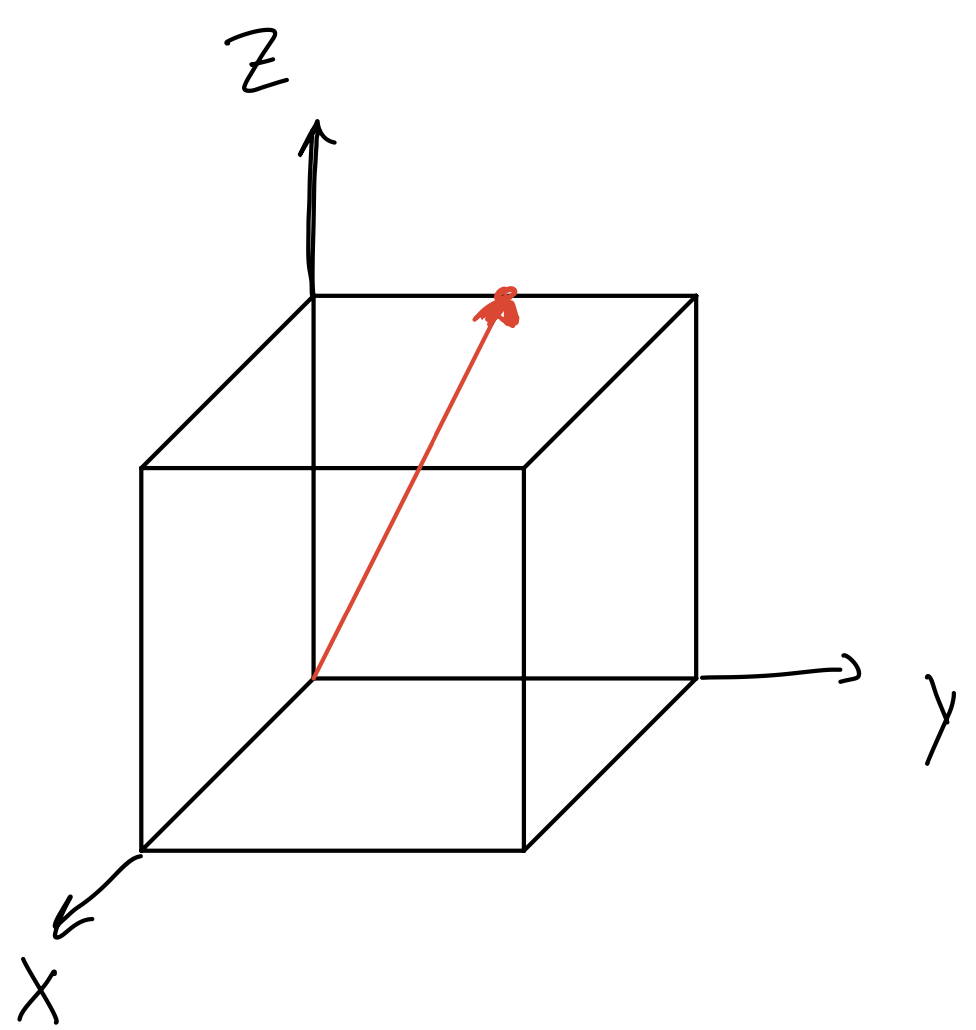
\includegraphics[width=0.5\textwidth]{3c.png}
\end{figure}

\subsection*{d. \small $\left[ 12\bar{1} \right]$}

\begin{figure}[H]
    \centering
    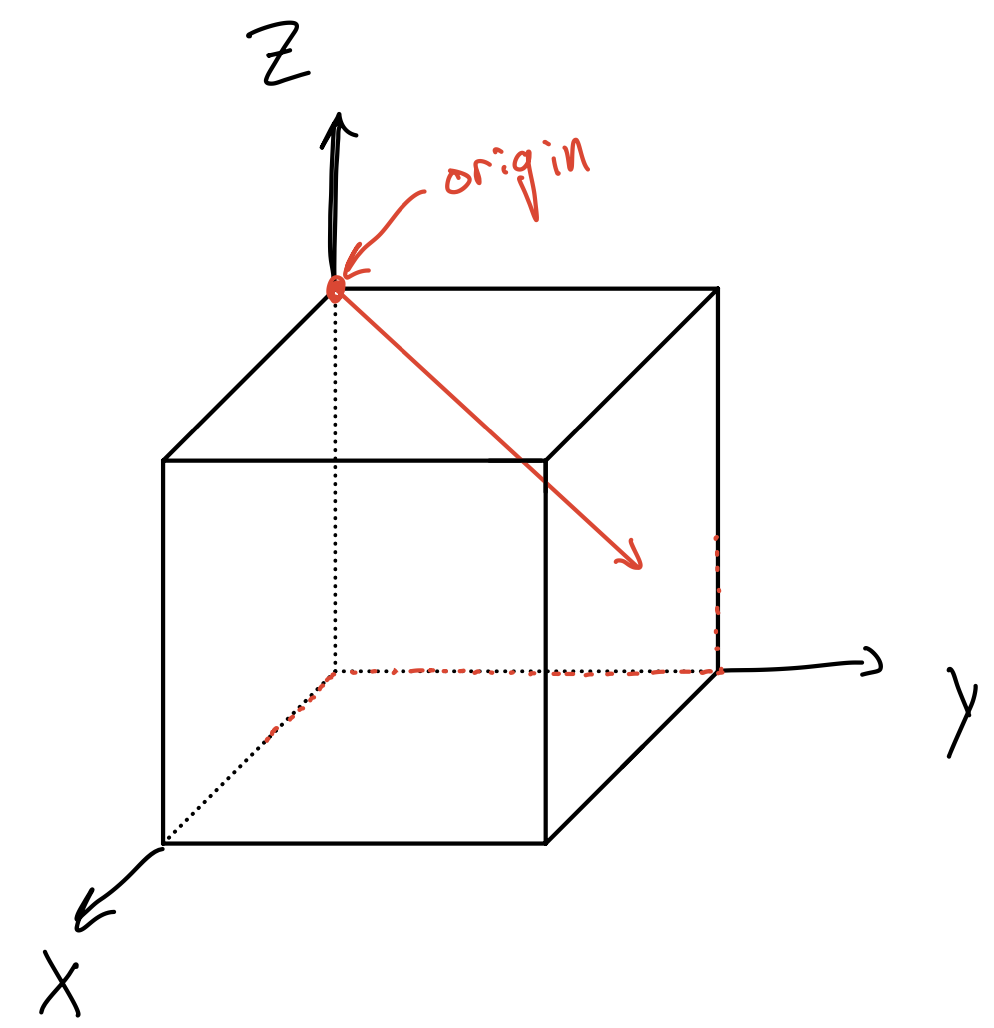
\includegraphics[width=0.5\textwidth]{3d.png}
\end{figure}

\section{Miller Indices: Planes}

\subsection*{a. (001)}

\begin{figure}[H]
    \centering
    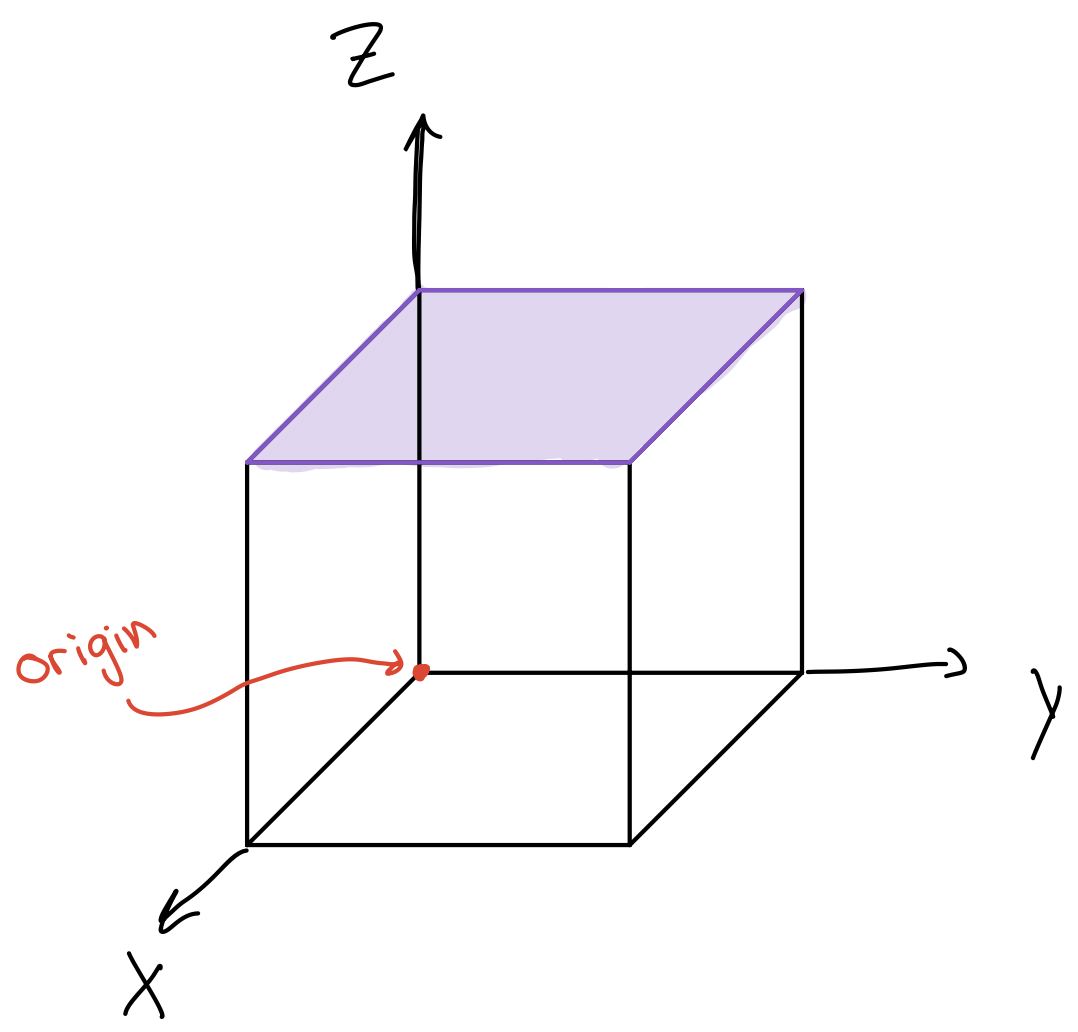
\includegraphics[width=0.5\textwidth]{4a.png}
\end{figure}

\subsection*{b. (201)}

\begin{figure}[H]
    \centering
    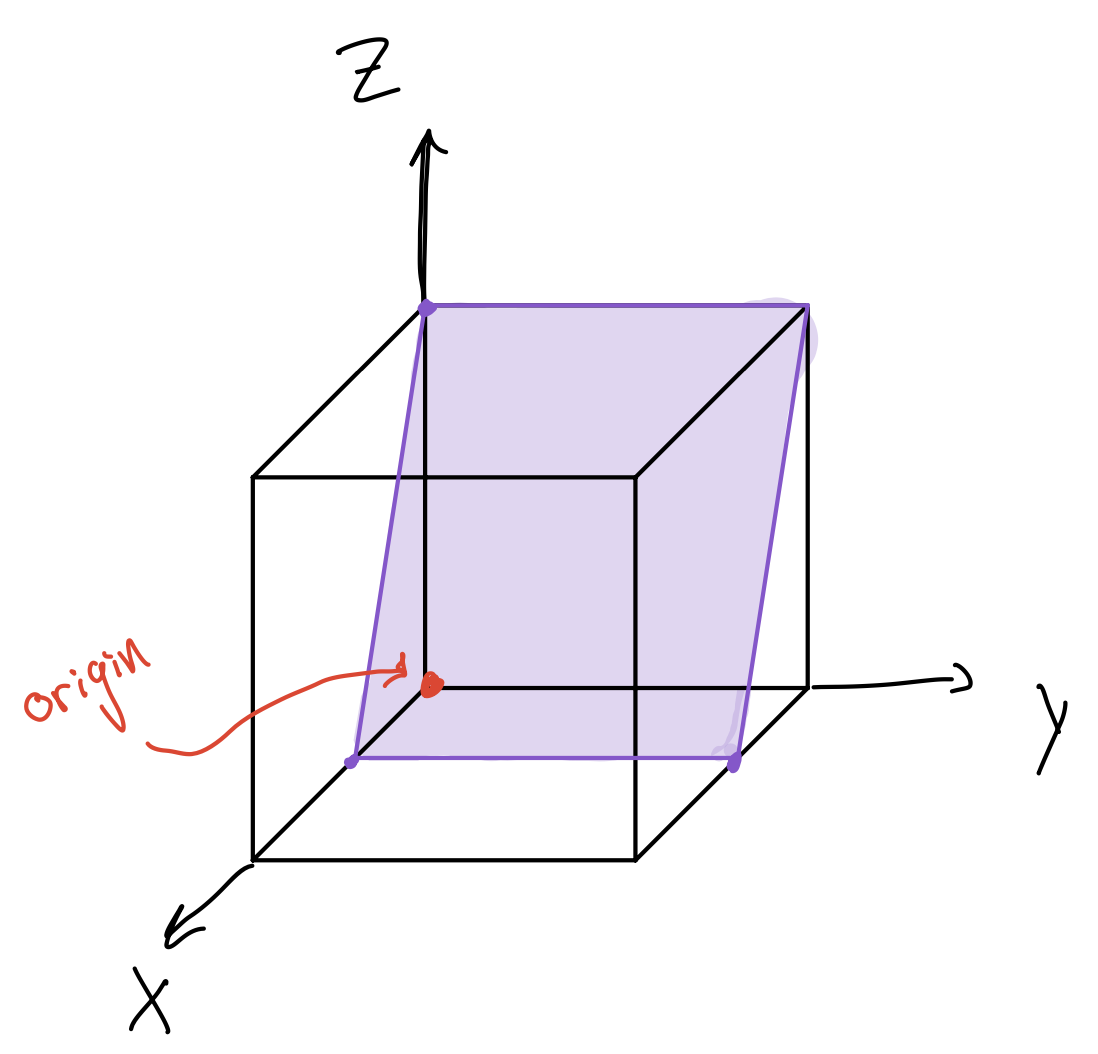
\includegraphics[width=0.5\textwidth]{4b.png}
\end{figure}

\subsection*{c. \small $\left(\bar{1}\bar{2}\bar{3}\right)$}

\begin{figure}[H]
    \centering
    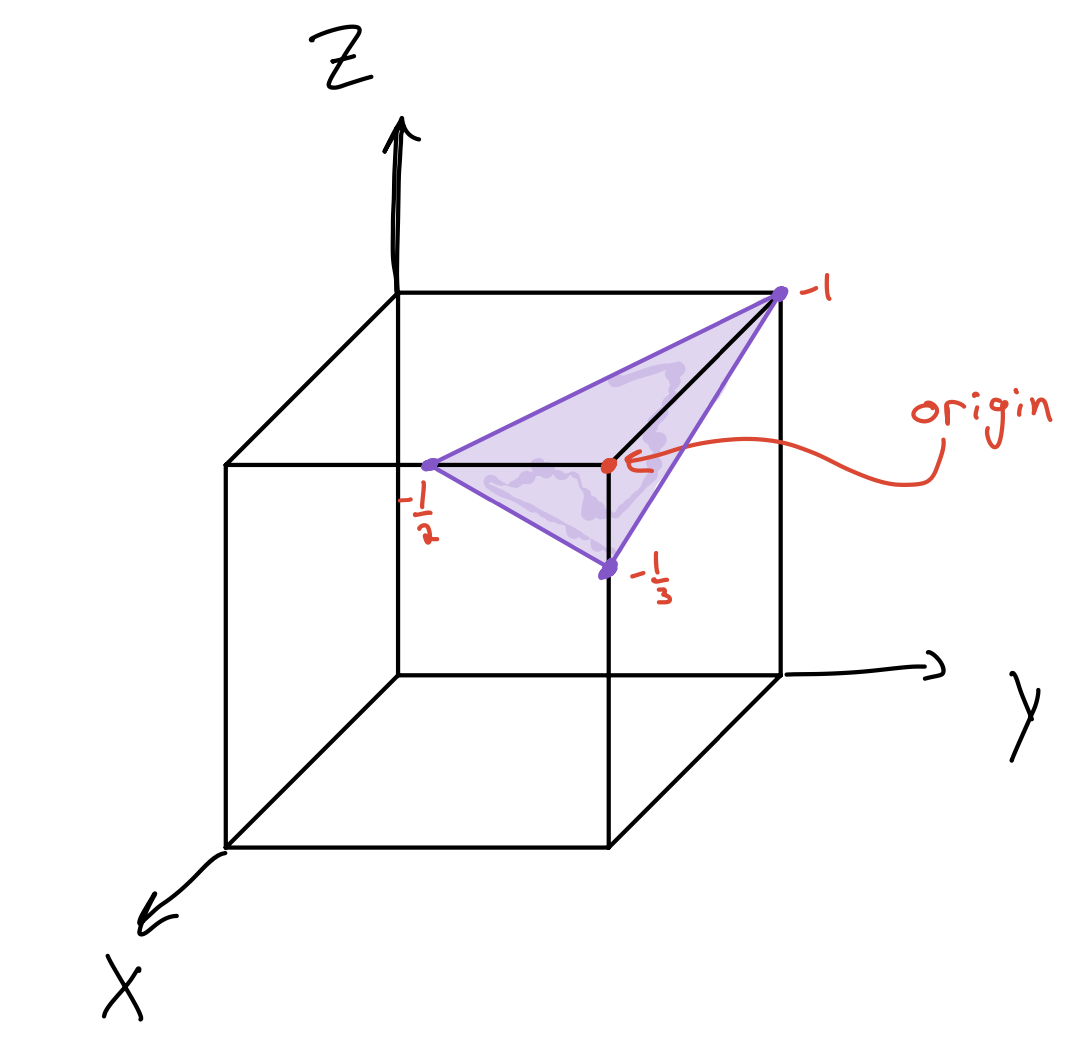
\includegraphics[width=0.5\textwidth]{4c.png}
\end{figure}

\subsection*{d. \small $(1\bar{1}\bar{2})$}

\begin{figure}[H]
    \centering
    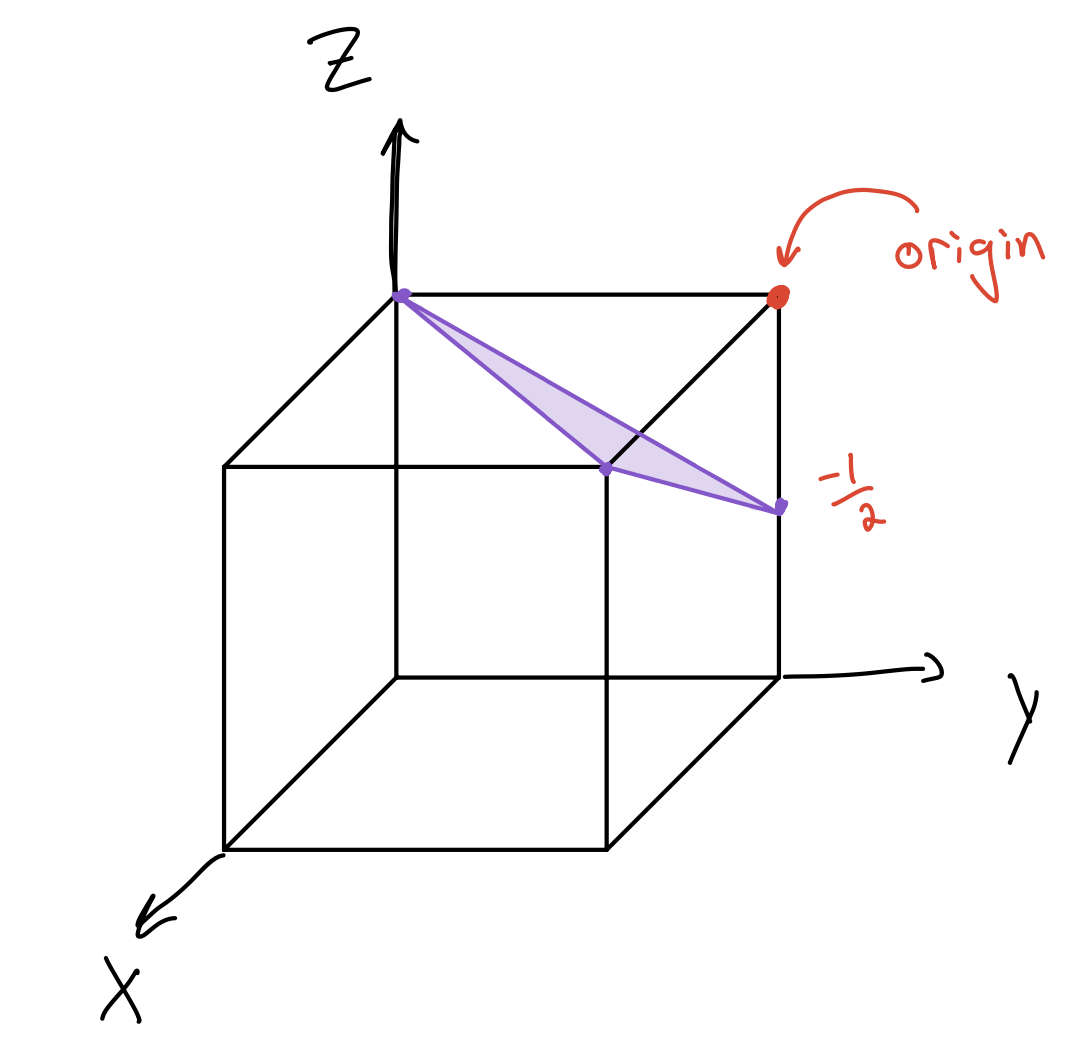
\includegraphics[width=0.5\textwidth]{4d.png}
\end{figure}


\end{document}